\section{Resultados}
Se encuestaron a 241 personas de más de 27 años de la ciudad de Culiacán —ver
apartado \nameref{sec:muestra}\pageref{sec:muestra}— de las cuales después de
hacer una valoración a las respuestas se tomaron únicamente 238 respuestas
válidas debido a la magnitud de las respuestas pues las preguntas abiertas no
tenían respuestas relevantes para el análisis, siendo respuestas como `porque
sí'. A continuación se presenta el análisis de la encuesta y las gráficas
obtenidas de las preguntas más relevantes. 

En la Figura~\ref{fig:grafica-23} se puede observar que el porcentaje de
aceptación de una aplicación de este tipo es realmente grande frente al que es
negativo. Este primer parámetro indica algo sumamente relevante —una viabilidad 
de proyecto positiva.

\begin{figure}[ht]
    \centering
    \fbox{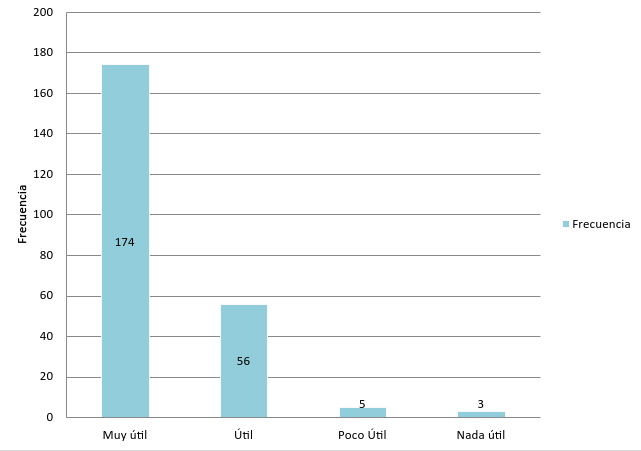
\includegraphics[width=0.6\textwidth]{imagenes/grafica-23.png}}
    \caption{Valores de aceptación de la aplicación, validando únicamente si
    sería de interés.}\label{fig:grafica-23}
\end{figure}

Mientas tanto, las siguientes dos preguntas están relacionados con el resultado
anterior, arrojando nuevos resultados —observados en las
Figuras~\ref{fig:grafica-24},~\ref{fig:grafica-25}— que permiten entender que
el consumidor está interesado en una aplicación de este tipo.

\begin{figure}[H]
    \centering
    \fbox{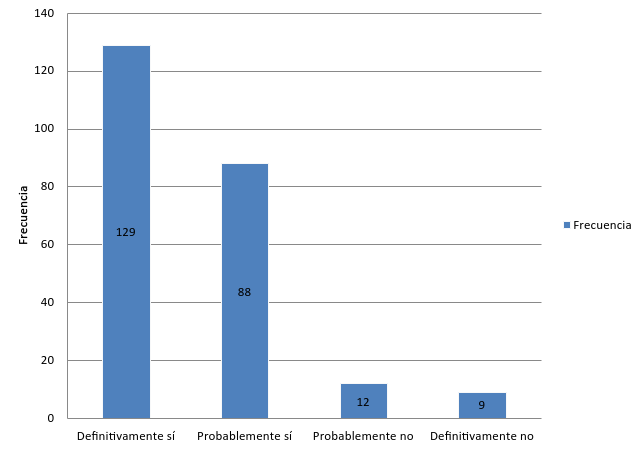
\includegraphics[width=0.6\textwidth]{imagenes/grafica-24.png}}
    \caption{Influencia en las decisiones de compra de dispositivos electrónicos
    del consumidor.}\label{fig:grafica-24}
\end{figure}

\begin{figure}[H]
    \centering
    \fbox{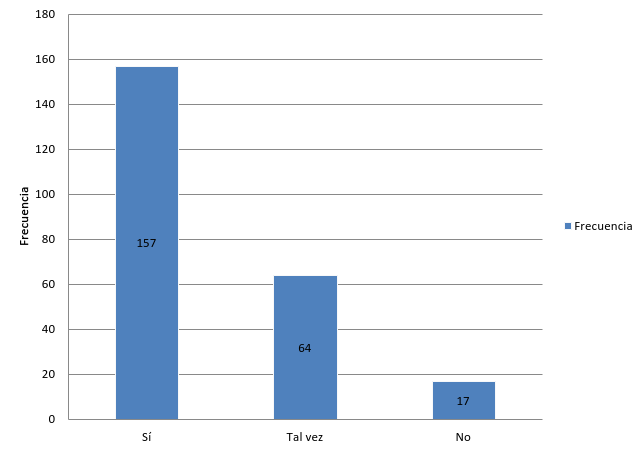
\includegraphics[width=0.6\textwidth]{imagenes/grafica-25.png}}
    \caption{Utilidad de la aplicación para toma de decisiones en la compra de los
    dispositivos electrónicos: smartphones, laptops.}\label{fig:grafica-25}
\end{figure}

Las respuestas de los encuestados indican que contar con una plataforma con la
información que la aplicación objetivo espera incluir sería de ayuda para las
próximas compras de los consumidores. El alto porcentaje de respuestas positivas
sobre la utilidad de una plataforma que centralice la información indica que
esta solución resulta cómoda para los usuarios y satisface una necesidad
importante: ahorrar tiempo en la búsqueda de información.

Las respuestas obtenidas sobre la viabilidad del proyecto de investigación y la
aplicación propuesta para combatir el consumo irracional y la obsolescencia
programada demuestran que esta iniciativa tendría un impacto significativo.
Principalmente, influiría en la forma en que las personas toman decisiones de
compra, al brindarles información relevante sobre cada producto de interés. Este
argumento se apoya en las siguientes preguntas, las cuales aportan datos
valiosos para inferir lo anterior. Al analizar las respuestas de los
encuestados, se evidencia que la problemática de la obsolescencia programada
está presente en la mayoría de los productos adquiridos a lo largo del tiempo,
especialmente si se comparan con los de hace 15 años. Esto respalda la idea de
que los productos actualmente están diseñados para dejar de funcionar después de
cierto periodo.

Se realizaron preguntas abiertas para entender más a fondo el comportamiento de
los consumidores, con el objetivo de sustentar lo dicho en la investigación, no
solo con referencias e investigaciones previas, sino también con lo que los
encuestados dijeron en relación con su contexto y situación. 

Las preguntas abiertas se diseñaron para explorar tanto la toma de decisiones
como las opiniones y percepciones personales sobre los hábitos de consumo. En
total, se plantearon 10 preguntas que abordan temas como: las razones para
adquirir un nuevo smartphone o laptop, el origen de la necesidad de compra, la
influencia de la publicidad en las decisiones, la comparación entre productos
actuales y los de hace 15 años, así como las opiniones sobre los materiales y
los cambios en la forma de consumir a lo largo del tiempo.

Respuestas como:
\begin{itemize}
    \item Ya tenía muchos años con el dispositivo previo —había perdido funcionalidad.
    \item La reparación era mas costosa que adquirir uno nuevo.
    \item Las actualizaciones ya no eran compatibles.
    \item La batería no duraba nada y era imposible de reemplazar.
    \item El modelo anterior que tenía empezó a responder muy lento. Se volvió complicado de usar. 
    \item Necesitaba una app que no era compatible con el modelo de mi celular.
\end{itemize}

Estas respuestas evidencian que la obsolescencia programada es un problema
relevante y vigente. Cambiar de dispositivo por razones tan simples como la
falta de actualizaciones o de almacenamiento resulta problemático, ya que
responde a intereses empresariales orientados a mantener las ganancias, sin
considerar las consecuencias ambientales y sociales. Con el tiempo, esto genera
una costumbre en los consumidores, que termina por aceptarse sin
cuestionamiento, especialmente debido al ritmo acelerado de la sociedad actual.

Una pregunta muy importante que demuestra cómo ha escalado la problemática es la
siguiente:

\noindent \textit{Imagina que tienes la oportunidad de comprar el teléfono que
deseas, pero debes elegir entre dos opciones respecto a los materiales con los
que fue fabricado: materiales con los estándares de calidad actuales o
materiales con los estándares de hace 15 años. ¿Cuál elegirías?  Explica tus
motivos.}

Las respuestas a la pregunta anterior pueden resumirse así: los consumidores
preferirían contar con la durabilidad de los dispositivos fabricados hace 15
años o más, pero integrando la tecnología actual. Muchos ya no confían
plenamente en los productos modernos, ya que han experimentado los cambios de
las distintas revoluciones industriales y el rápido avance tecnológico. De
hecho, la llegada de la cuarta revolución industrial ha provocado un incremento
masivo en la compra de dispositivos electrónicos cada vez que surge una
innovación. Las  respuestas son en su mayoría a favor de las tecnologías del
pasado porque se reconoce su durabilidad, sin embargo, los mismos consumidores
aceptan que hoy en día se está a la vanguardia con el avance tecnológico,
reconociendo la importancia de disfrutar de las comodidades que los dispositivos
modernos ofrecen. El hecho de conocer estas paralelidades entre el presente y el
pasado hace ver que se debe buscar un equilibrio entre las tecnologías pasadas,
sinónimos de durabilidad, confianza y persistencia, y las presentes, sinónimos
de innovación, seguridad y eficiencia.

El 83\% de los encuestados observados en la Figura~\ref{fig:grafica-16} consideran que las cosas están hechas para desecharse;
el objetivo es cambiar esa mentalidad, no se busca regresar al pasado de forma
negativa, sino que las compras se realicen con la información necesaria para
tomar decisiones con la menor cantidad de sesgos posibles, así como la noción de
que las decisiones tienen consecuencias —como el derecho a reparar. Si se busca
que la voz de los consumidores sea escuchada, es posible lograr cambios, pero
esto no ocurre de manera espontánea. Se requiere información; por ello, si se
proporciona a los consumidores una herramienta que les permita acceder a
información relevante, podrán transformar sus hábitos y, en conjunto, influir en
la sociedad actual.

\begin{figure}[H]
    \centering
    \fbox{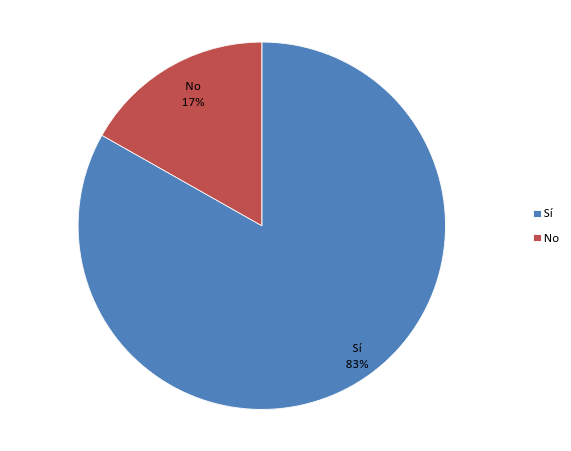
\includegraphics[width=0.6\textwidth]{imagenes/grafica-16.png}}
    \caption{Percepción de durabilidad de dispositivos actuales.}\label{fig:grafica-16}
\end{figure}

El proyecto dentro de todos sus matices tiene uno muy importante, informar. 
En las Figuras~\ref{fig:grafica-03},~\ref{fig:grafica-01},~\ref{fig:grafica-07} se
puede observar con mayor porcentaje el desconocimiento de la
población ante términos importantes para los consumidores, lo que hace ver que
sí es relevante informar pues sabiendo qué engloba un término, una
situación o una problemática podemos comenzar para combatirla. Informando de esto
se comienza a cuestionar el sistema y a decidir con valor. 

\begin{figure}[H]
    \centering
    \fbox{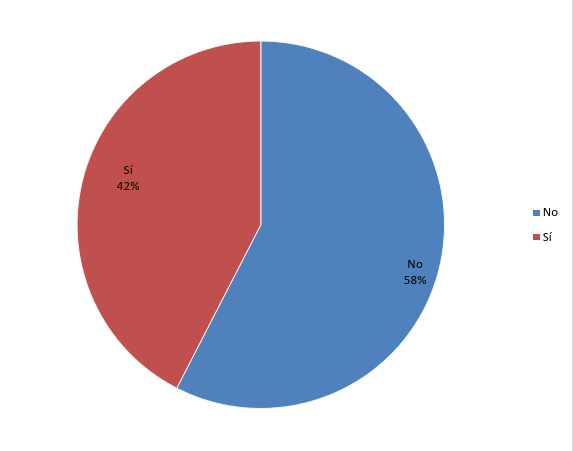
\includegraphics[width=0.6\textwidth]{imagenes/grafica-01.png}}
    \caption{Conocimiento general del concepto de obsolescencia programada.}\label{fig:grafica-01}
\end{figure}

\begin{figure}[H]
    \centering
    \fbox{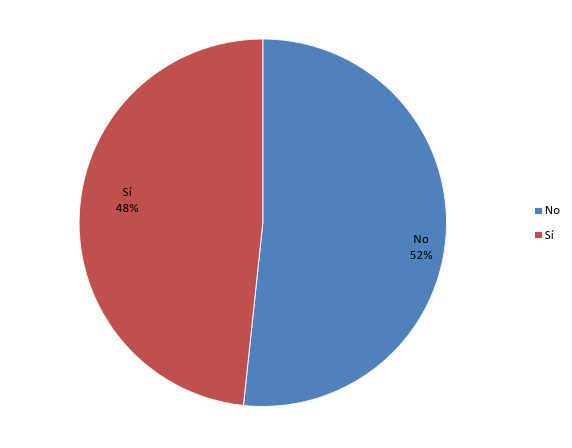
\includegraphics[width=0.6\textwidth]{imagenes/grafica-03.png}}
    \caption{Conocimiento general del concepto de economía circular.}\label{fig:grafica-03}
\end{figure}

\begin{figure}[H]
    \centering
    \fbox{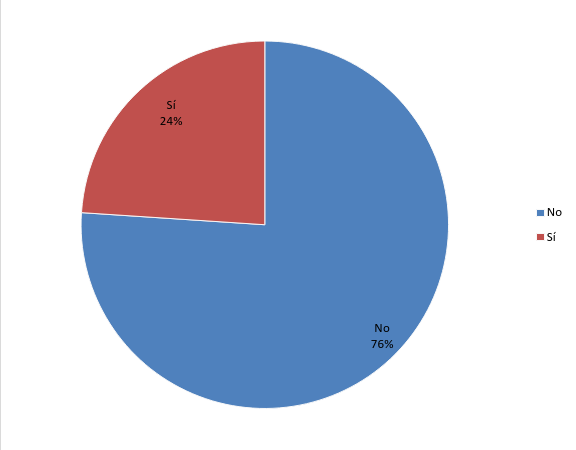
\includegraphics[width=0.6\textwidth]{imagenes/grafica-07.png}}
    \caption{Conocimiento general del concepto de greenwashing.}\label{fig:grafica-07}
\end{figure}

